% !TEX root = ./Basilisk-SunlineEphem-20181204.tex


\begin{figure}[h]
	\centerline{
		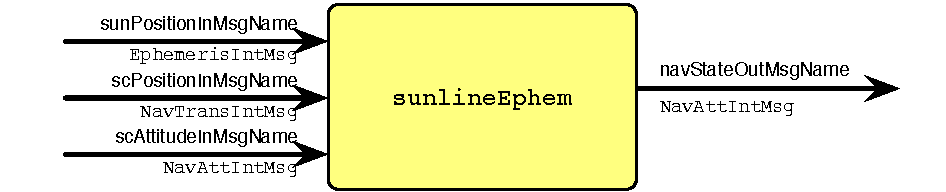
\includegraphics{Figures/moduleIO}
	}
	\caption{Sample Figure Inclusion.}
	\label{fig:Fig1}
\end{figure}


\section{Model Description}

The sunline ephemeris module is responsible for calculating a sunline heading based exclusively on ephemeris data. This provides a estimate for the sun heading without relying of filtering results from the course sun sensors. 

%\subsection{Equations}
The math is straightforward; subtract the position of the sun from the position of the spacecraft, and divide it by its norm, to compute the sun heading in the inertial frame $\hat{\bm{r}}_{h_N}$. 
\begin{equation}
	{}^{\mathcal N}\hat{\bm{r}}_{S/B} = \frac{\bm{\bm{r}}_{\text{sun}}-\bm{\bm{r}}_{sc}}{|\bm{\bm{r}}_{\text{sun}} - \bm{\bm{r}}_{sc}|}
\end{equation}
Rotate the unit vector into the body frame by multiplying it by the appropriate direction cosine matrix defined by the spacecraft's attitude properties, $\bm{\sigma}$. 
\begin{equation}
	{}^{\mathcal N}\hat{\bm{r}}_{S/B} = [BN(\bm{\sigma})]*{}^{\mathcal{N}}\hat{\bm{r}}_{S/B}
\end{equation}

